\documentclass[12pt,a4paper]{article}

\usepackage[T1]{fontenc}
\usepackage[utf8]{inputenc}
\usepackage[polish]{babel}
\usepackage{lmodern}
\usepackage{geometry}
\usepackage{booktabs}
\usepackage{array}
\usepackage{amsmath}
\usepackage{listings}
\usepackage{xcolor}
\usepackage{hyperref}
\usepackage{float}
\usepackage{caption}
\usepackage{multirow}
\usepackage{pdfpages}
\usepackage{graphicx}

\geometry{margin=2.5cm}

\hypersetup{colorlinks=true, linkcolor=black, urlcolor=blue}

\lstset{
  basicstyle=\ttfamily\small,
  keywordstyle=\color{blue},
  commentstyle=\color{gray},
  stringstyle=\color{orange},
  breaklines=true,
  frame=single,
  language=Python,
  showstringspaces=false,
}

\begin{document}


\includepdf[pages=1]{title-page.pdf}

\newpage
\tableofcontents
\newpage

% ============================================================
\section{Opis projektu}
% ============================================================

Tematem projektu jest implementacja zmodyfikowanej wersji algorytmu indukcji reguł AQ,
w której do oceny kompleksu dodawanego w kolejnych iteracjach wykorzystywany jest
osobny zbiór walidacyjny.

Celem projektu jest porównanie klasycznej wersji algorytmu AQ z wersją zmodyfikowaną
i sprawdzenie, czy ocenianie kompleksów na osobnym zbiorze walidacyjnym może ograniczyć
przeuczenie oraz poprawić wyniki na nowych danych, przy czym efekt ten może zależeć
od charakterystyki zbioru.
Projekt zakłada implementację obu wersji algorytmu, przeprowadzenie eksperymentów
na trzech zbiorach danych oraz analizę uzyskanych wyników.

% ============================================================
\section{Podstawy teoretyczne}
% ============================================================

\subsection{Algorytm AQ}

Algorytm AQ (Algorithm Quasi-optimal) należy do klasy algorytmów indukcji reguł
i służy do budowy klasyfikatorów w postaci zestawu reguł logicznych
\cite{michalski1969, michalski1983}.
Reguły mają postać:

\[
\texttt{JEŚLI } c_1 \wedge c_2 \wedge \ldots \wedge c_k \;\texttt{ TO } \mathit{klasa} = K
\]

gdzie każdy warunek $c_i$ ogranicza wartość jednego atrybutu do wybranego podzbioru
dopuszczalnych wartości.
Zbiór takich warunków nazywany jest \textbf{kompleksem}.
Kompleks \emph{pokrywa} dany przykład, jeśli wszystkie jego warunki są spełnione.

\subsubsection*{Klasyczna wersja algorytmu}

Dla każdej klasy docelowej $K$ algorytm wykonuje następujące kroki:

\begin{enumerate}
  \item Wybierz losowy przykład pozytywny (należący do klasy $K$) jako ziarno
        (\emph{seed}).
  \item Generuj \textbf{gwiazdę} -- zbiór kompleksów pokrywających ziarno
        i wykluczających przykłady negatywne. Kandydaci są specjalizowani poprzez
        dodawanie kolejnych warunków, tak aby żaden z kompleksów nie pokrywał
        żadnego przykładu negatywnego.
  \item Spośród kandydatów wybierz \textbf{najlepszy kompleks} według miary jakości
        (w implementacji: $F_1$ wyważone między precyzją a pokryciem).
  \item Utwórz regułę na podstawie wybranego kompleksu i usuń ze zbioru niepokrytych
        wszystkie przykłady pozytywne pokryte tą regułą.
  \item Powtarzaj kroki 1--4, aż wszystkie przykłady pozytywne zostaną pokryte
        lub zostanie osiągnięty limit reguł.
\end{enumerate}

\subsubsection*{Przeszukiwanie wiązką (ang.\ \emph{beam search})}

Ponieważ przestrzeń możliwych kompleksów jest wykładniczo duża, w kroku generacji
gwiazdy stosuje się \textbf{przeszukiwanie wiązką} o szerokości $b$.
W każdym kroku specjalizacji utrzymywany jest zbiór co najwyżej $b$ najlepiej
ocenionych kandydatów, a pozostałe są odrzucane.
Szerokość wiązki kontroluje kompromis między jakością rozwiązania a kosztem
obliczeniowym.

\subsection{Zmodyfikowana wersja ze zbiorem walidacyjnym}

W klasycznej wersji algorytmu ocena kandydatów odbywa się na
\textbf{tym samym zbiorze treningowym}, na którym kompleksy zostały zbudowane.
Może to prowadzić do sytuacji analogicznej do nadmiernego dopasowania
(\emph{overfitting}): wybierane są kompleksy ściśle dopasowane do danych
treningowych, które niekoniecznie uogólniają się na nowe dane.

\medskip
\noindent\textbf{Proponowana modyfikacja} polega na rozdzieleniu dwóch ról zbioru danych:

\begin{itemize}
  \item \textbf{Zbiór treningowy} -- służy do generowania i specjalizowania kompleksów
        (wykluczania przykładów negatywnych). Struktura kompleksów jest zatem
        wyznaczana na podstawie danych treningowych.
  \item \textbf{Zbiór walidacyjny} -- służy wyłącznie do oceny i rankingu kandydatów
        w każdym kroku przeszukiwania wiązką. Najlepszy kompleks w danej iteracji
        jest wybierany na podstawie jego $F_1$ obliczonego na zbiorze walidacyjnym.
\end{itemize}

Mechanizm ten jest koncepcyjnie zbliżony do techniki wczesnego zatrzymania
(\emph{early stopping}) \cite{bishop2006} stosowanej przy trenowaniu sieci neuronowych --
zewnętrzny sygnał jakości zastępuje ocenę opartą wyłącznie na danych uczących.

\subsubsection*{Kluczowy fragment implementacji}

Metoda \texttt{\_score\_set\_for\_class} decyduje, który zbiór zostanie użyty
do oceny kandydatów w danej iteracji -- zwraca \texttt{"train"} dla wariantu
klasycznego lub \texttt{"validation"} dla wariantu zmodyfikowanego
(z zabezpieczeniem na wypadek braku przykładów walidacyjnych dla danej klasy):

\begin{lstlisting}
def _score_set_for_class(self, target_class):
    if self.variant != "validation":
        return "train"       # wariant klasyczny
    if self._validation_label_masks[target_class].bit_count() == 0:
        return "train"       # fallback: brak przykladow walidacyjnych dla klasy
    return "validation"      # wariant zmodyfikowany
\end{lstlisting}

Następnie metoda \texttt{\_score\_candidate} na podstawie zwróconej wartości
wybiera odpowiednie maski bitowe i oblicza $\mathit{TP}$, $\mathit{FP}$
oraz $F_1$ na właściwym zbiorze:

\begin{lstlisting}
if score_set == "validation":
    full_mask       = self._full_validation_mask
    condition_masks = self._validation_condition_masks
    label_mask      = self._validation_label_masks[target_class]
else:
    full_mask       = self._full_train_mask
    condition_masks = self._train_condition_masks
    label_mask      = self._train_label_masks[target_class]
\end{lstlisting}

Zastosowanie masek bitowych zamiast iteracji po przykładach znacząco przyspiesza
obliczenia dla dużych zbiorów danych (np.\ Nursery z ponad 12\,000 przykładami).

\subsection{Metryki oceny}
\label{sec:metryki}

Do porównania wariantów użyto następujących miar:

\begin{itemize}
  \item \textbf{Accuracy} -- odsetek poprawnie sklasyfikowanych przykładów.
  \item \textbf{Precision, Recall, F1 (ważone)} -- miary ważone wsparciem klas
        (ang.\ \emph{weighted}): każda klasa jest uwzględniana proporcjonalnie
        do liczby jej przykładów; miarodajne przy nierównomiernym rozkładzie klas.
        W tabelach oznaczane skrótem \emph{Prec.}, \emph{Rec.}, \emph{F1\textsubscript{W}}.
  \item \textbf{Macro F1} -- średnia arytmetyczna $F_1$ po klasach bez ważenia;
        szczególnie czuła na klasy mniejszościowe.
  \item \textbf{Luka train--test} -- różnica między wynikiem
        na zbiorze treningowym a testowym; bezpośrednia miara stopnia przeuczenia.
        W tabelach oznaczana jako \emph{Luka train--test}.
  \item \textbf{Liczba reguł i średnia złożoność} -- miary zwięzłości i
        interpretowalności modelu.
\end{itemize}

Wszystkie wyniki są uśrednione po 5 niezależnych losowych podziałach danych
(ziarna 0--4). Podawane są wartości średnie wraz z odchyleniem standardowym
populacyjnym ($\mu \pm \sigma$).

% ============================================================
\section{Implementacja}
% ============================================================

Projekt zaimplementowano w języku \textbf{Python 3} bez użycia zewnętrznych
bibliotek uczenia maszynowego (takich jak scikit-learn czy pandas).
Cały kod indukcji reguł, podziału danych i ewaluacji napisano od podstaw,
korzystając wyłącznie z biblioteki standardowej.

Implementacja składa się z dwóch plików:

\begin{itemize}
  \item \texttt{aq\_experiments.py} -- zawiera klasę \texttt{AQClassifier}
        implementującą oba warianty algorytmu AQ, klasy pomocnicze
        (\texttt{Rule}, \texttt{CandidateStats}), stratyfikowany podział danych
        (\texttt{stratified\_split}) oraz funkcję ewaluacji
        (\texttt{evaluate\_predictions}).
  \item \texttt{evaluate.py} -- skrypt uruchamiający eksperymenty porównawcze
        na wskazanych zbiorach danych, zbierający wyniki per-seed
        i zapisujący je do pliku CSV.
\end{itemize}

Do generowania losowych podziałów danych wykorzystano generator pseudolosowy
z biblioteki standardowej Pythona (\texttt{random.Random}), inicjalizowany
kolejnymi ziarenami (0--4), co zapewnia pełną reprodukowalność wyników.

Kluczowe decyzje implementacyjne:

\begin{itemize}
  \item \textbf{Maski bitowe} -- każdy przykład jest reprezentowany jako bit
        w liczbie całkowitej. Operacje AND na maskach zastępują pętle po przykładach,
        co daje wielokrotne przyspieszenie dla dużych zbiorów.
  \item \textbf{Pamięć podręczna wyników} (\emph{score cache}) -- wyniki
        \texttt{\_score\_candidate} są zapamiętywane w słowniku indeksowanym
        krotką \texttt{(complex, target\_class, score\_set)}, eliminując
        wielokrotne obliczenia dla tych samych kandydatów.
  \item \textbf{Wariant algorytmu} -- parametr \texttt{variant} klasy
        \texttt{AQClassifier} przyjmuje wartość \texttt{"classic"} lub
        \texttt{"validation"}, co pozwala uruchamiać oba warianty tym samym kodem.
  \item \textbf{Klasyfikacja} -- przy predykcji stosuje się zasadę pierwszej
        pasującej reguły z rankingiem według score, precyzji, pokrycia i złożoności.
        Jeśli żadna reguła nie pasuje, zwracana jest klasa dominująca ze zbioru
        treningowego.
\end{itemize}

% ============================================================
\section{Zbiory danych}
% ============================================================

W projekcie wykorzystano trzy zbiory danych z repozytorium UCI Machine Learning
Repository \cite{dua2019}, różniące się rozmiarem, liczbą atrybutów i trudnością klasyfikacji.

\subsection{Car Evaluation}

\begin{itemize}
  \item \textbf{Liczba przykładów:} 1728
  \item \textbf{Liczba atrybutów:} 6 (wszystkie kategoryczne):
        \texttt{buying}, \texttt{maint}, \texttt{doors},
        \texttt{persons}, \texttt{lug\_boot}, \texttt{safety}
  \item \textbf{Klasy:} \texttt{unacc} (1210), \texttt{acc} (384),
        \texttt{good} (69), \texttt{vgood} (65)
\end{itemize}

Zbiór posiada silnie nierównomierny rozkład klas -- klasa \texttt{unacc} stanowi
około 70\% wszystkich przykładów. Jest to naturalny benchmark dla algorytmów
indukcji reguł ze względu na czysto symboliczny charakter danych.

\subsection{Mushrooms}

\begin{itemize}
  \item \textbf{Liczba przykładów:} 8124
  \item \textbf{Liczba atrybutów:} 22 (wszystkie kategoryczne)
  \item \textbf{Klasy:} \texttt{p} -- trujący (3916), \texttt{e} -- jadalny (4208)
\end{itemize}

Zbiór opisuje cechy morfologiczne grzybów. Klasy są dobrze zbalansowane.
Dane zawierają silne korelacje atrybutów z klasą (m.in.\ zapach, kolor wysypu
zarodników), co sprawia, że problem jest potencjalnie łatwy do pokrycia zwartymi
regułami logicznymi.

\subsection{Nursery}

\begin{itemize}
  \item \textbf{Liczba przykładów:} 12960
  \item \textbf{Liczba atrybutów:} 8 (wszystkie kategoryczne):
        \texttt{parents}, \texttt{has\_nurs}, \texttt{form}, \texttt{children},
        \texttt{housing}, \texttt{finance}, \texttt{social}, \texttt{health}
  \item \textbf{Klasy:} \texttt{not\_recom} (4320), \texttt{priority} (4266),
        \texttt{spec\_prior} (4044), \texttt{very\_recom} (328),
        \texttt{recommend} (2)
\end{itemize}

Największy ze zbiorów, zawierający dwie skrajnie mniejszościowe klasy
(\texttt{recommend}: 2 przykłady, \texttt{very\_recom}: 328 przykładów).
Dane pochodzą z systemu wspomagania decyzji przyjęć do żłobków.
Ze względu na rozmiar zbioru czas jednego uruchomienia przy szerokości wiązki
$b = 30$ był zbyt długi, aby przeprowadzić pełną serię 5 podziałów w rozsądnym
czasie -- eksperymenty dotyczące wpływu szerokości wiązki przeprowadzono dla Nursery
przy $b = 10$ (zob.\ sekcja~\ref{sec:bw}).

\subsection{Podział danych}

We wszystkich eksperymentach zastosowano \textbf{stratyfikowany podział} danych,
gwarantujący zachowanie proporcji klas w każdym ze zbiorów.
Domyślny podział:

\[
\text{treningowy} = 60\%, \quad \text{walidacyjny} = 20\%, \quad \text{testowy} = 20\%
\]

% ============================================================
\section{Eksperymenty i wyniki}
% ============================================================

We wszystkich tabelach kolumny \emph{Prec.}, \emph{Rec.} i \emph{F1\textsubscript{W}}
oznaczają miary ważone wsparciem klas (zob.\ sekcja~\ref{sec:metryki}).
We wszystkich eksperymentach użyto limitu 200 reguł na klasę
(\texttt{-{}-max-rules-per-class 200}).

\subsection{Eksperyment 1 -- Porównanie wariantów (wyniki główne)}

\textbf{Parametry:} szerokość wiązki $b = 30$, podział 60/20/20\%,
limit reguł 200, 5 podziałów losowych (ziarna 0--4).

\subsubsection*{Car Evaluation}

\begin{table}[H]
\centering
\caption{Car Evaluation -- jakość na zbiorze testowym ($\mu \pm \sigma$, $n=5$)}
\begin{tabular}{lcccc}
\toprule
Wariant & Accuracy & Prec. & Rec. & Macro F1 \\
\midrule
Klasyczny   & $0.8740 \pm 0.0108$ & $0.8691 \pm 0.0105$ & $0.8740 \pm 0.0108$ & $0.6827 \pm 0.0236$ \\
Walidacyjny & $0.8699 \pm 0.0208$ & $0.8623 \pm 0.0251$ & $0.8699 \pm 0.0208$ & $0.6491 \pm 0.0642$ \\
\bottomrule
\end{tabular}
\end{table}

\begin{table}[H]
\centering
\caption{Car Evaluation -- przeuczenie i złożoność modelu ($\mu \pm \sigma$, $n=5$)}
\begin{tabular}{lcccc}
\toprule
Wariant & Train acc & Luka train--test & Liczba reguł & Śr. warunki \\
\midrule
Klasyczny   & $1.0000 \pm 0.0000$ & $0.1260 \pm 0.0108$ & $149.8 \pm 6.7$ & $4.73 \pm 0.04$ \\
Walidacyjny & $1.0000 \pm 0.0000$ & $0.1301 \pm 0.0208$ & $169.4 \pm 8.5$ & $4.87 \pm 0.04$ \\
\bottomrule
\end{tabular}
\end{table}

Na zbiorze Car Evaluation oba warianty osiągają zbliżoną dokładność testową
($0.8740$ vs $0.8699$). Wariant klasyczny uzyskuje wyższe Macro F1
($0.6827$ vs $0.6491$), co wskazuje na lepsze pokrycie klas mniejszościowych.
Wariant walidacyjny generuje o 13\% więcej reguł (169 vs 150) przy nieco wyższej
złożoności warunkowej. Wariancja wyników wariantu walidacyjnego jest niemal
dwukrotnie większa, co świadczy o większej wrażliwości na konkretny podział danych.

\subsubsection*{Mushrooms}

\begin{table}[H]
\centering
\caption{Mushrooms -- jakość na zbiorze testowym ($\mu \pm \sigma$, $n=5$)}
\begin{tabular}{lcccc}
\toprule
Wariant & Accuracy & Prec. & Rec. & Macro F1 \\
\midrule
Klasyczny   & $1.0000 \pm 0.0000$ & $1.0000 \pm 0.0000$ & $1.0000 \pm 0.0000$ & $1.0000 \pm 0.0000$ \\
Walidacyjny & $1.0000 \pm 0.0000$ & $1.0000 \pm 0.0000$ & $1.0000 \pm 0.0000$ & $1.0000 \pm 0.0000$ \\
\bottomrule
\end{tabular}
\end{table}

\begin{table}[H]
\centering
\caption{Mushrooms -- przeuczenie i złożoność modelu ($\mu \pm \sigma$, $n=5$)}
\begin{tabular}{lcccc}
\toprule
Wariant & Train acc & Luka train--test & Liczba reguł & Śr. warunki \\
\midrule
Klasyczny   & $1.0000 \pm 0.0000$ & $0.0000 \pm 0.0000$ & $25.8 \pm 1.2$ & $3.05 \pm 0.01$ \\
Walidacyjny & $1.0000 \pm 0.0000$ & $0.0000 \pm 0.0000$ & $26.4 \pm 2.1$ & $3.01 \pm 0.02$ \\
\bottomrule
\end{tabular}
\end{table}

Na zbiorze Mushrooms oba warianty osiągają doskonałą klasyfikację (accuracy = 1.0000)
przy zerowej luce train--test i minimalnej liczbie reguł (ok.\ 26).
Zbiór ten zawiera silne, deterministyczne zależności, które algorytm AQ odkrywa
niezależnie od wariantu oceny kompleksów.

\subsubsection*{Nursery}

\begin{table}[H]
\centering
\caption{Nursery -- jakość na zbiorze testowym ($b=30$, $\mu \pm \sigma$, $n=5$)}
\begin{tabular}{lcccc}
\toprule
Wariant & Accuracy & Prec. & Rec. & Macro F1 \\
\midrule
Klasyczny   & $0.9633 \pm 0.0023$ & $0.9647 \pm 0.0025$ & $0.9633 \pm 0.0023$ & $0.7947 \pm 0.0798$ \\
Walidacyjny & $0.9649 \pm 0.0039$ & $0.9662 \pm 0.0032$ & $0.9649 \pm 0.0039$ & $0.8353 \pm 0.0864$ \\
\bottomrule
\end{tabular}
\end{table}

\begin{table}[H]
\centering
\caption{Nursery -- przeuczenie i złożoność modelu ($b=30$, $\mu \pm \sigma$, $n=5$)}
\begin{tabular}{lcccc}
\toprule
Wariant & Train acc & Luka train--test & Liczba reguł & Śr. warunki \\
\midrule
Klasyczny   & $0.9974 \pm 0.0008$ & $0.0342 \pm 0.0025$ & $461.8 \pm 3.9$ & $5.14 \pm 0.02$ \\
Walidacyjny & $0.9954 \pm 0.0004$ & $0.0305 \pm 0.0042$ & $481.0 \pm 3.9$ & $5.22 \pm 0.02$ \\
\bottomrule
\end{tabular}
\end{table}

Nursery jest jedynym zbiorem, na którym wariant walidacyjny osiąga mierzalnie
lepsze wyniki testowe: accuracy $0.9649$ vs $0.9633$ oraz Macro F1 $0.8353$
vs $0.7947$ (poprawa o $+0.040$). Jednocześnie luka train--test jest mniejsza
($0.0305$ vs $0.0342$), co potwierdza ograniczenie przeuczenia. Obserwacja ta jest
szczególnie istotna, gdyż Nursery zawiera skrajnie mniejszościowe klasy --
zbiór walidacyjny pozwala lepiej oceniać kompleksy pod kątem ich
uogólnienia na rzadkich klasach.

Duże odchylenie standardowe Macro F1 dla obu wariantów ($\sigma \approx 0.08$,
widoczne na rysunku~\ref{fig:macro_f1}) jest zjawiskiem oczekiwanym i wynika
z dwóch czynników. Po pierwsze, przy zaledwie $n = 5$ podziałach losowych
każdy pojedynczy podział ma duży wpływ na wartość średnią. Po drugie,
klasa \texttt{recommend} liczy tylko 2 przykłady w całym zbiorze --
w zależności od podziału trafia ona w całości do zbioru treningowego
albo testowego, co powoduje skokowe zmiany Macro F1 między podziałami.
Szerokość słupków błędów odzwierciedla zatem niestabilność miary, a nie
niestabilność algorytmu.

\begin{figure}[H]
  \centering
  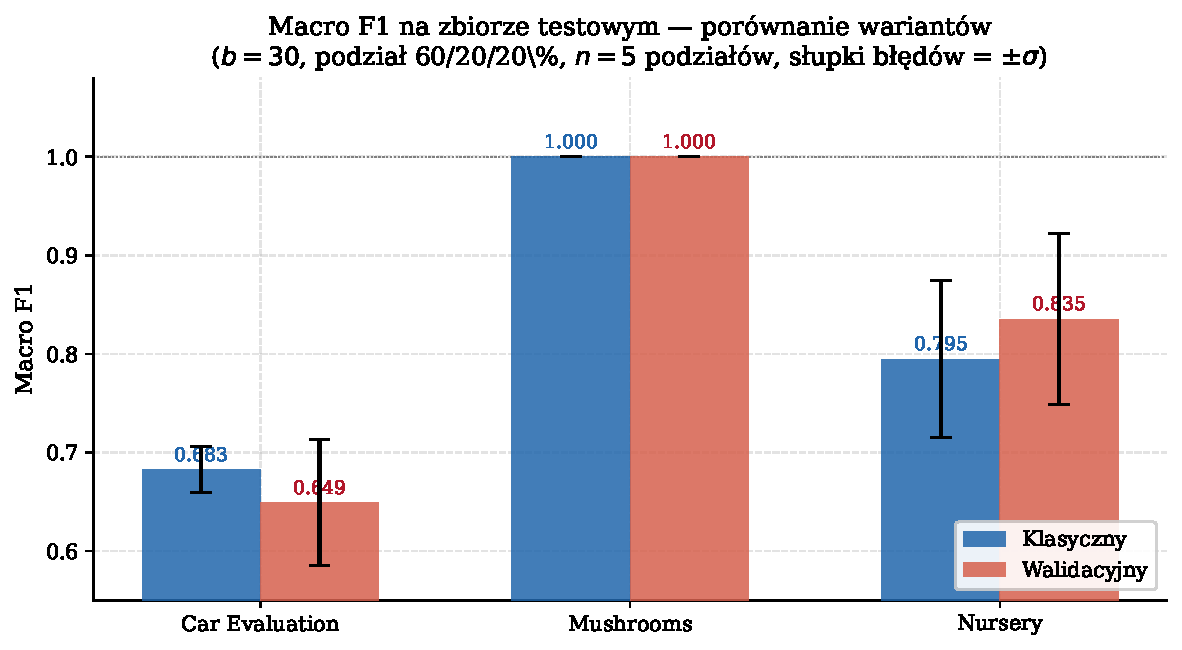
\includegraphics[width=0.82\textwidth]{plot1_macro_f1.pdf}
  \caption{Macro F1 na zbiorze testowym dla obu wariantów algorytmu na trzech
           zbiorach danych ($b=30$, podział 60/20/20\%, $n=5$;
           słupki błędów oznaczają $\pm\sigma$).}
  \label{fig:macro_f1}
\end{figure}

\subsection{Eksperyment 2 -- Wpływ szerokości wiązki}
\label{sec:bw}

Badano wpływ parametru $b \in \{10, 30, 60\}$ dla zbiorów Car Evaluation
i Mushrooms przy podziale 60/20/20\%.
Na zbiorze Nursery ze względu na czas obliczeń przy $b = 30$ użyto $b = 10$
jako jedynej wartości bazowej (tabela~\ref{tab:nursery-bw10}).

\begin{table}[H]
\centering
\caption{Wpływ szerokości wiązki -- Car Evaluation ($\mu \pm \sigma$, $n=5$)}
\label{tab:bw-car}
\begin{tabular}{cccccc}
\toprule
$b$ & Wariant & Accuracy & Macro F1 & Luka train--test & Liczba reguł \\
\midrule
\multirow{2}{*}{10}
  & Klasyczny   & $0.8717 \pm 0.0145$ & $0.6726 \pm 0.0420$ & $0.1283 \pm 0.0145$ & $150.2 \pm 8.7$ \\
  & Walidacyjny & $0.8728 \pm 0.0215$ & $0.6577 \pm 0.0701$ & $0.1272 \pm 0.0215$ & $170.2 \pm 9.9$ \\
\midrule
\multirow{2}{*}{30}
  & Klasyczny   & $0.8740 \pm 0.0108$ & $0.6827 \pm 0.0236$ & $0.1260 \pm 0.0108$ & $149.8 \pm 6.7$ \\
  & Walidacyjny & $0.8699 \pm 0.0208$ & $0.6491 \pm 0.0642$ & $0.1301 \pm 0.0208$ & $169.4 \pm 8.5$ \\
\midrule
\multirow{2}{*}{60}
  & Klasyczny   & $0.8740 \pm 0.0151$ & $0.6790 \pm 0.0417$ & $0.1260 \pm 0.0151$ & $150.4 \pm 6.4$ \\
  & Walidacyjny & $0.8775 \pm 0.0230$ & $0.6719 \pm 0.0643$ & $0.1225 \pm 0.0230$ & $168.4 \pm 10.4$ \\
\bottomrule
\end{tabular}
\end{table}

\begin{table}[H]
\centering
\caption{Nursery -- oba warianty przy $b=10$ ($\mu \pm \sigma$, $n=5$)}
\label{tab:nursery-bw10}
\begin{tabular}{lcccc}
\toprule
Wariant & Accuracy & Macro F1 & Luka train--test & Liczba reguł \\
\midrule
Klasyczny   & $0.9588 \pm 0.0038$ & $0.7579 \pm 0.0695$ & $0.0354 \pm 0.0043$ & $465.8 \pm 3.1$ \\
Walidacyjny & $0.9601 \pm 0.0038$ & $0.8343 \pm 0.0874$ & $0.0308 \pm 0.0038$ & $481.2 \pm 5.2$ \\
\bottomrule
\end{tabular}
\end{table}

Szerokość wiązki nie ma istotnego wpływu na accuracy testową -- różnice między
$b = 10$, $b = 30$ i $b = 60$ mieszczą się w granicach odchylenia standardowego
dla obu wariantów na zbiorze Car Evaluation. Wariant walidacyjny generuje
konsekwentnie o ok.\ 12--13\% więcej reguł niż klasyczny niezależnie od wartości $b$.
Przy $b = 60$ wariant walidacyjny uzyskuje nieznacznie wyższą accuracy
($0.8775$ vs $0.8740$) i niższą lukę train--test ($0.1225$ vs $0.1260$),
co sugeruje, że szersza wiązka daje większy wybór kandydatów i pozwala
zbiorowi walidacyjnemu wybrać bardziej ogólne kompleksy.
Na zbiorze Nursery przy $b = 10$ wzorzec jest taki sam jak przy $b = 30$:
wariant walidacyjny osiąga wyższe Macro F1 ($0.8343$ vs $0.7579$)
i mniejszą lukę train--test ($0.0308$ vs $0.0354$).

\begin{figure}[H]
  \centering
  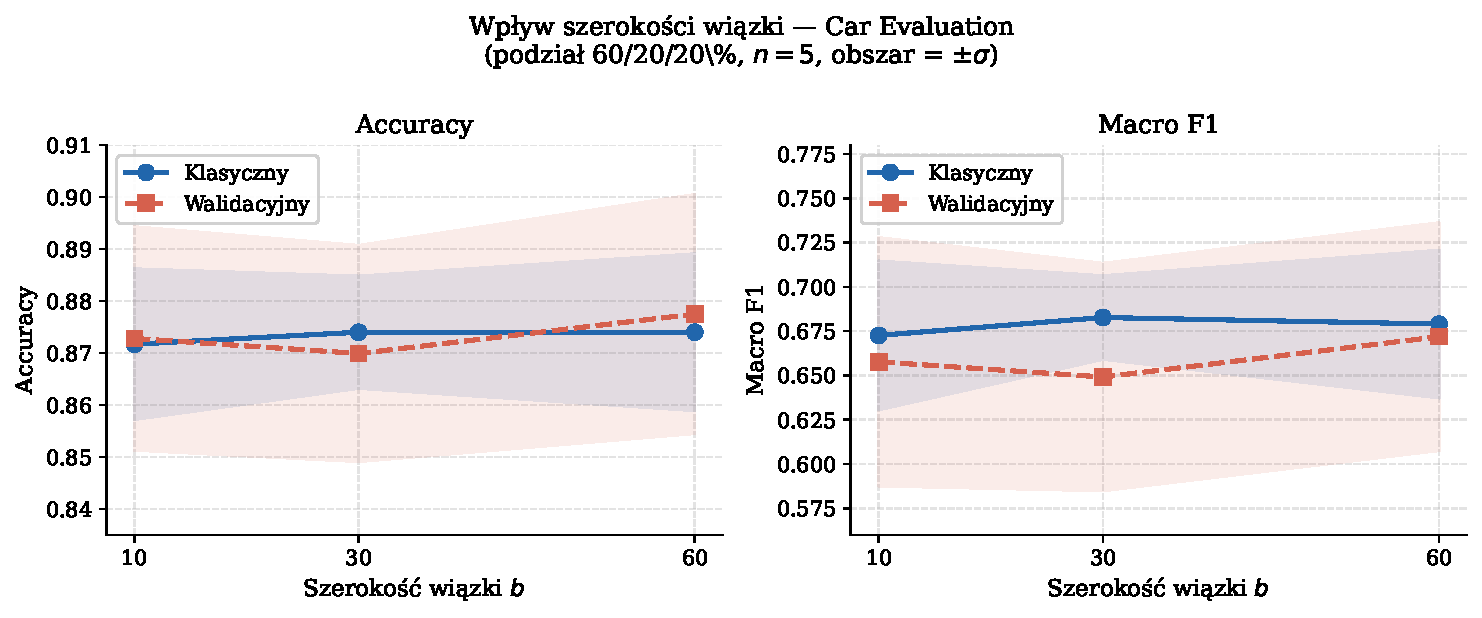
\includegraphics[width=0.92\textwidth]{plot2_beam_width.pdf}
  \caption{Wpływ szerokości wiązki $b$ na accuracy i Macro F1 - Car Evaluation
           (podział 60/20/20\%, $n=5$; obszar zacieniowany = $\pm\sigma$).}
  \label{fig:beam_width}
\end{figure}

\subsection{Eksperyment 3 -- Wpływ rozmiaru zbioru walidacyjnego}

Badano wpływ proporcji zbioru walidacyjnego przy $b = 30$ i limicie reguł 200.
Rozmiar zbioru testowego pozostał stały (20\%); zmieniano proporcje między
zbiorem treningowym a walidacyjnym.

\begin{table}[H]
\centering
\caption{Wpływ rozmiaru zbioru walidacyjnego -- Car Evaluation ($\mu \pm \sigma$, $n=5$)}
\label{tab:val-car}
\begin{tabular}{ccccc}
\toprule
Podział tr/val & Wariant & Accuracy & Macro F1 & Liczba reguł \\
\midrule
\multirow{2}{*}{70\% / 10\%}
  & Klasyczny   & $0.8844 \pm 0.0102$ & $0.6771 \pm 0.0592$ & $170.2 \pm 11.6$ \\
  & Walidacyjny & $0.8838 \pm 0.0201$ & $0.6648 \pm 0.0804$ & $190.0 \pm 11.4$ \\
\midrule
\multirow{2}{*}{60\% / 20\%}
  & Klasyczny   & $0.8740 \pm 0.0108$ & $0.6827 \pm 0.0236$ & $149.8 \pm 6.7$ \\
  & Walidacyjny & $0.8699 \pm 0.0208$ & $0.6491 \pm 0.0642$ & $169.4 \pm 8.5$ \\
\midrule
\multirow{2}{*}{50\% / 30\%}
  & Klasyczny   & $0.8647 \pm 0.0119$ & $0.6354 \pm 0.0627$ & $130.4 \pm 6.0$ \\
  & Walidacyjny & $0.8647 \pm 0.0218$ & $0.6685 \pm 0.0732$ & $147.6 \pm 7.8$ \\
\bottomrule
\end{tabular}
\end{table}

Zmniejszenie zbioru treningowego (na rzecz większego walidacyjnego) obniża accuracy
obu wariantów -- mniejszy zbiór treningowy ogranicza liczbę wygenerowanych reguł
(130 vs 150 vs 170), zmniejszając pokrycie przestrzeni cech.

Interesującą obserwacją jest zachowanie Macro F1: przy podziale 50/30\% wariant
walidacyjny uzyskuje wyższe Macro F1 niż klasyczny ($0.6685$ vs $0.6354$),
podczas gdy przy podziale 70/10\% sytuacja jest odwrotna ($0.6648$ vs $0.6771$).
Wskazuje to, że większy zbiór walidacyjny poprawia ocenę rzadkich klas,
bez istotnego wpływu na accuracy.

\begin{figure}[H]
  \centering
  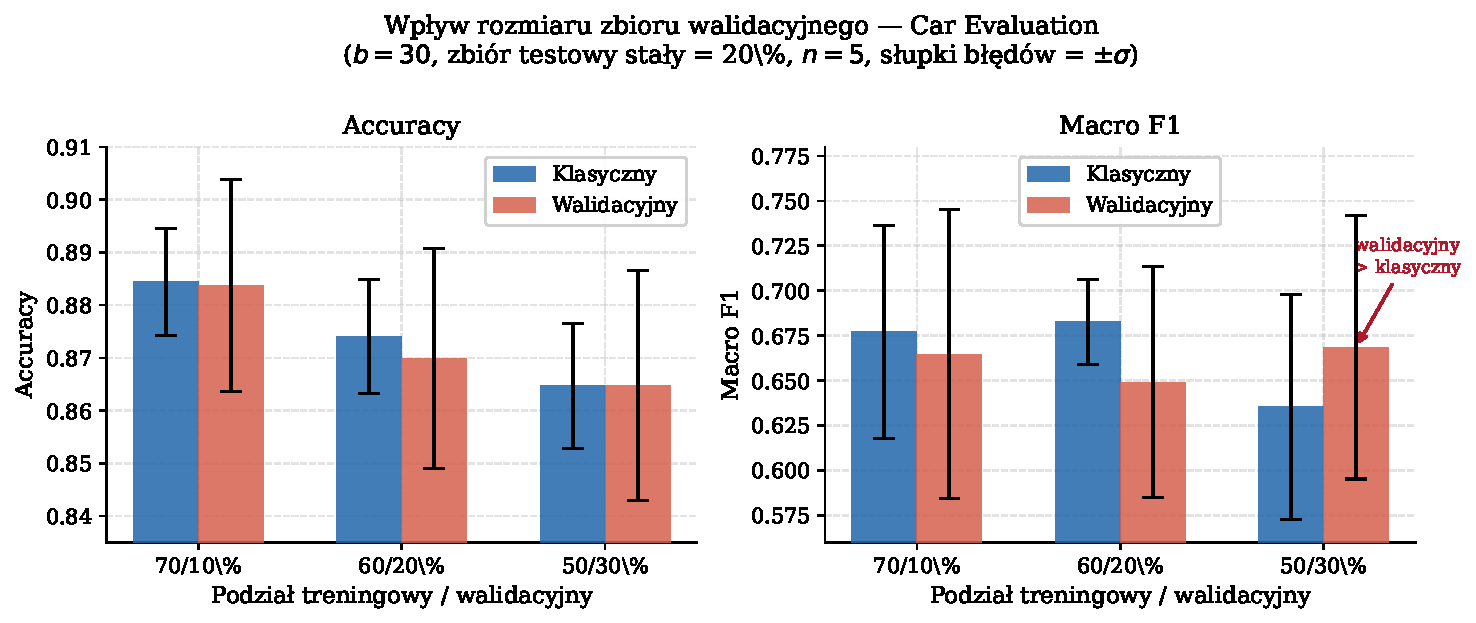
\includegraphics[width=0.92\textwidth]{plot3_val_size.pdf}
  \caption{Wpływ rozmiaru zbioru walidacyjnego na accuracy i Macro F1 - Car Evaluation
           ($b=30$, zbiór testowy stały = 20\%, $n=5$;
           strzałka wskazuje konfigurację, w której wariant walidacyjny przewyższa
           klasyczny pod względem Macro F1).}
  \label{fig:val_size}
\end{figure}

% ============================================================
\section{Wnioski i podsumowanie}
% ============================================================

\begin{table}[H]
\centering
\caption{Zestawienie wyników głównego eksperymentu ($b=30$, podział 60/20/20\%)}
\begin{tabular}{llccc}
\toprule
Zbiór & Wariant & Accuracy & Macro F1 & Luka train--test \\
\midrule
\multirow{2}{*}{Car Evaluation}
  & Klasyczny   & $0.8740 \pm 0.0108$ & $0.6827 \pm 0.0236$ & $0.1260 \pm 0.0108$ \\
  & Walidacyjny & $0.8699 \pm 0.0208$ & $0.6491 \pm 0.0642$ & $0.1301 \pm 0.0208$ \\
\midrule
\multirow{2}{*}{Mushrooms}
  & Klasyczny   & $1.0000 \pm 0.0000$ & $1.0000 \pm 0.0000$ & $0.0000 \pm 0.0000$ \\
  & Walidacyjny & $1.0000 \pm 0.0000$ & $1.0000 \pm 0.0000$ & $0.0000 \pm 0.0000$ \\
\midrule
\multirow{2}{*}{Nursery}
  & Klasyczny   & $0.9633 \pm 0.0023$ & $0.7947 \pm 0.0798$ & $0.0342 \pm 0.0025$ \\
  & Walidacyjny & $0.9649 \pm 0.0039$ & $0.8353 \pm 0.0864$ & $0.0305 \pm 0.0042$ \\
\bottomrule
\end{tabular}
\end{table}

Na podstawie przeprowadzonych eksperymentów sformułowano następujące wnioski:

\begin{enumerate}

  \item \textbf{Wpływ modyfikacji zależy od charakterystyki zbioru danych.}
        Wariant walidacyjny przynosi wyraźne korzyści na zbiorze Nursery --
        dużym, wieloklasowym, z silnie nierównomiernym rozkładem:
        accuracy $+0.0016$, Macro F1 $+0.0406$, mniejsza luka train--test
        ($0.0305$ vs $0.0342$).
        Na zbiorze Car Evaluation różnice są marginalne i niejednoznaczne,
        natomiast na zbiorze Mushrooms, gdzie dane są niemal liniowo separowalne
        regułami logicznymi, oba warianty dają identyczne wyniki (accuracy = 1.0).
        Modyfikacja ma zatem potencjał przede wszystkim w scenariuszach
        z wieloma klasami, szumem lub nakładającymi się obszarami decyzyjnymi.

  \item \textbf{Wariant walidacyjny generuje więcej reguł.}
        We wszystkich konfiguracjach wariant walidacyjny tworzy konsekwentnie więcej
        reguł niż klasyczny: ok.\ 12--13\% dla Car Evaluation i ok.\ 3--4\%
        dla Nursery. Wynika to z faktu, że kompleksy wybrane na podstawie
        zbioru walidacyjnego są zazwyczaj bardziej zachowawcze (wyższa precyzja,
        mniejsze pokrycie), przez co w każdej iteracji usuwają mniej przykładów
        z puli niepokrytych, wymagając większej liczby reguł do pokrycia całości.

  \item \textbf{Wariant walidacyjny cechuje się większą wariancją wyników.}
        Odchylenie standardowe wyników wariantu walidacyjnego jest konsekwentnie
        wyższe niż klasycznego. Jest to koszt uzależnienia rankingu kandydatów
        od stosunkowo małego zbioru walidacyjnego, który może nie być
        reprezentatywny dla wszystkich klas przy każdym podziale.

  \item \textbf{Większy zbiór walidacyjny sprzyja klasom mniejszościowym.}
        Przy podziale 50/30\% wariant walidacyjny osiąga wyższe Macro F1 niż
        klasyczny ($0.6685$ vs $0.6354$), przy identycznej accuracy ($0.8647$).
        Większy zbiór walidacyjny lepiej reprezentuje rzadkie klasy i pozwala
        na korzystniejszy wybór kompleksów dla klas mniejszościowych.

  \item \textbf{Szerokość wiązki ma marginalne znaczenie.}
        W zakresie $b \in \{10, 30, 60\}$ nie zaobserwowano istotnych różnic
        w accuracy. Większa wiązka nieznacznie sprzyja wariantowi walidacyjnemu
        (niższa luka train--test przy $b = 60$), lecz efekt nie jest duży
        w stosunku do odchylenia standardowego wyników.

\end{enumerate}

\subsubsection*{Ograniczenia metodologiczne}

Przeprowadzone eksperymenty mają kilka istotnych ograniczeń, które należy
wziąć pod uwagę przy interpretacji wyników:

\begin{itemize}
  \item \textbf{Mała liczba podziałów ($n = 5$).} Uśrednianie po zaledwie 5
        losowych podziałach danych daje stosunkowo szerokie przedziały ufności.
        Różnice między wariantami na poziomie $|\Delta\text{acc}| < 0.005$
        (Car Evaluation) mogą nie być istotne statystycznie -- weryfikacja
        wymagałaby testu, np.\ Wilcoxona dla prób sparowanych lub co najmniej
        $n = 30$ podziałów.
  \item \textbf{Brak testów istotności statystycznej.} Wyniki prezentowane są
        wyłącznie jako $\mu \pm \sigma$; nie przeprowadzono formalnych testów
        hipotez. Sformułowane wnioski mają charakter eksploracyjny.
  \item \textbf{Ograniczony zakres hiperparametrów.} Przeszukiwano jedynie
        trzy wartości szerokości wiązki i trzy proporcje podziału danych;
        inne kombinacje mogłyby ujawnić inne zależności.
  \item \textbf{Jeden typ funkcji oceny.} Zarówno podczas budowy gwiazdy,
        jak i przy ocenie na zbiorze walidacyjnym używano miary $F_1$.
        Użycie innych miar (np.\ samej precyzji lub pokrycia) mogłoby
        inaczej ukształtować zachowanie wariantu walidacyjnego.
\end{itemize}

\medskip
\noindent\textbf{Podsumowanie.}
Zmodyfikowana wersja algorytmu AQ z oceną kompleksów na zbiorze walidacyjnym
jest poprawnie zaimplementowana i działa zgodnie z założeniami projektu.
Wyniki eksperymentów wskazują, że modyfikacja przynosi mierzalne korzyści
przede wszystkim na zbiorach dużych i wieloklasowych z nierównomiernym rozkładem klas
(Nursery), gdzie ogranicza przeuczenie i poprawia Macro F1.
Na zbiorach z silnymi deterministycznymi zależnościami lub mniejszych
różnice między wariantami są marginalne.
Kosztem modyfikacji jest większa liczba generowanych reguł i wyższa wrażliwość
na podział danych, co przy małej liczbie podziałów utrudnia jednoznaczne
wnioskowanie statystyczne.

% ============================================================
\begin{thebibliography}{9}

\bibitem{michalski1969}
Michalski, R.S. (1969).
\textit{On the quasi-minimal solution of the general covering problem}.
Proceedings of the 5th International Symposium on Information Processing (FCIP 69),
Bled, Yugoslavia, vol.\ A3, pp.\ 125--128.

\bibitem{michalski1983}
Michalski, R.S. (1983).
A theory and methodology of inductive learning.
W: Michalski, R.S., Carbonell, J.G., Mitchell, T.M. (red.),
\textit{Machine Learning: An Artificial Intelligence Approach}, vol.\ 1,
pp.\ 83--134. Tioga Publishing, Palo Alto, CA.

\bibitem{dua2019}
Dua, D., Graff, C. (2019).
\textit{UCI Machine Learning Repository}.
University of California, Irvine, School of Information and Computer Sciences.
Dostępne pod adresem: \url{https://archive.ics.uci.edu}

\bibitem{bishop2006}
Bishop, C.M. (2006).
\textit{Pattern Recognition and Machine Learning}.
Springer, New York, NY.

\end{thebibliography}

\end{document}
